\documentclass[12pt,english]{article}
\usepackage{geometry}
\geometry{verbose,letterpaper,tmargin=2.4cm,bmargin=2.4cm,lmargin=2.4cm,rmargin=2.4cm}
\usepackage[T1]{fontenc}
\usepackage{lmodern}
\usepackage{amssymb,amsmath}
\usepackage{ifxetex,ifluatex}
\usepackage[round]{natbib}
\bibliographystyle{plainnat}
\usepackage{graphicx}
\usepackage{caption}
\usepackage{subcaption}
\usepackage{brush_style}
\usepackage{setspace}
\usepackage{lineno}
\usepackage{listings}
\begin{document}

\renewcommand{\thefigure}{S\arabic{figure}}
 \renewcommand{\thetable}{S\arabic{table}}

\appendix
\section{Appendix}
In Appendix \ref{stab}, we provide the details for assessing the persistence of a population with an integrodifference model and we discuss the effect of the harvesting function on population persistence.  In Appendix \ref{sep}, we provide the details for assessing population persistence with separable dispersal kernels.  In Appendix \ref{gausapp} and \ref{sinapp}, we derive expressions for the critical harvesting rate and rate of environmental shift for Gaussian and sinuosoidal dispersal kernels.  In Appendix \ref{approxcrit}, we derive approximate expressions for these critical rates. In Appendix \ref{MPA} we provide details on differences between small and large MPA simulations. In Appendix \ref{rock}, we parameterize our model for black rockfish ($Sebastes melanops$)in the California Current and demonstrate that results for  parameters  are qualitatively similar to results  presented in the main text. 


\subsection{Determining stability \label{stab}}
Let $n_t(x)$ be the number of adults at position $x$ at time $t$, let $k(x)$ be a dispersal kernel describingt the probability of a larva traveling a distance $x$, let $f(n)$ be the recruitment function describing the number of offspring that settle and survive in juvenile population of size $n$, let $R_0$ be the intrinsic growth rate of the population, and let $g(n)$ be the harvesting function describing the number of adults harvested from a population of size $n$.  In the absence of harvesting, the integrodifference model describing the population over time is given by 

\begin{equation} n_{t+1}(x)=\int_{-L/2+ct}^{L/2+ct}k(x-y)R_0f(n_t(y))dy \label{integro} \end{equation}
as described in \citet{ZhouKot2011}.  With the addition of harvesting, the model becomes

\begin{equation} n_{t+1}(x)=\int_{-L/2+ct}^{L/2+ct}k(x-y)R_0g(f(n_t(y)))dy. \label{integro} \end{equation}

In evaluating persistence, we apply the methods of \citet{ZhouKot2011} to the new model, Equation 2.  A traveling pulse is a solution such that population size relative to location within the patch (rather than absolute position) is constant over time, i.e. 

\begin{equation*}
n^*(\overline{x}_t)\equiv n^*(x-ct)=n_t(x),   \label{trav} 
\end{equation*}
where $\overline{x}_t\equiv x-ct$ gives position relative to the patch. 

The integrodifference equation (\ref{integro}) gives us an expression for $n^*$:

\begin{align}
n^*(\overline{x}_{t+1})&=n_{t+1}(x) \notag
\\ &=\int_{-L/2+ct}^{L/2+ct}k(x-y)R_0g(f(n_t(y)))dy \notag
\\ &=\int_{-L/2+ct}^{L/2+ct}k(x-\overline{y}_t-ct)R_0g(f(n^*(\overline{y}_t)))dy \notag
\\ &=\int_{-L/2+ct}^{L/2+ct}k(\overline{x}_t-\overline{y}_t)R_0g(f(n^*(\overline{y}_t)))dy \notag
\\ \Rightarrow n^*(\overline{x}_t-c)&=\int_{-L/2+ct}^{L/2+ct}k(\overline{x}_t-\overline{y}_t)R_0g(f(n^*(\overline{y}_t)))dy \notag
%\\n^*(\overline{x}-c)&=\int_{-L/2}^{L/2}k(\overline{x}-\overline{y})f(n^*(\overline{y})-g(n^*(\overline{y})))d\overline y \notag
\\ \Rightarrow n^*(\overline{x}_t)&=\int_{-L/2}^{L/2}k(\overline{x}_t+c-\overline{y}_t)R_0g(f(n^*(\overline{y}_t)))d\overline y_t  \label{pulse}
\end{align}
As long as $f(0)=0$, there is a trivial solution to this problem where $n^*(\overline{x})\equiv 0$ for all $\overline{x}$, i.e., there is a trivial traveling pulse with no adults in it.  If the trivial traveling pulse is unstable, even very small populations will persist or grow and avoid crashing back to the trivial pulse.  To evaluate the stability of a traveling pulse, we introduce a small perturbation to the traveling pulse $n^*(\overline{x})$ and see if this perturbation grows or shrinks over time:

\begin{align}
n_t(x)&=n^*(\overline{x}_t)+\xi_t(x) \notag
\\ \Rightarrow \xi_{t+1}(x)&=n_{t+1}(x)-n^*(\overline{x}_{t+1}) \notag
\\&=n_{t+1}(x)-n^*(\overline{x}_{t}-c) \notag
\\ &=\int_{-L/2+ct}^{L/2+ct}k(x-y)R_0g(f(n_t(y)))dy-\int_{-L/2}^{L/2}k(\overline{x}_{t}-\overline{y}_t)R_0g(f(n^*(\overline{y}_t)))d\overline y_t \text{ using (\ref{pulse})} \notag
%\\ &=\int_{-L/2+ct}^{L/2+ct}k(x-y)f(n_t(y)-g(n_t(y)))dy-\int_{-L/2}^{L/2}k(\overline{x}_{t}-\overline{y}_t)f(n^*(\overline{y}_t)-g(n^*(\overline{y}_t))d\overline y_t \notag
\\ &=\int_{-L/2+ct}^{L/2+ct}k(x-y)R_0g(f(n_t(y)))dy-\int_{-L/2+ct}^{L/2+ct}k(x-ct-(y-ct))R_0g(f(n^*(\overline{y}_t)))d\overline y_t \notag
\\ &=\int_{-L/2+ct}^{L/2+ct}k(x-y)R_0g(f(n_t(y)))dy-\int_{-L/2+ct}^{L/2+ct}k(x-y)R_0g(f(n^*(\overline{y}_t)))d\overline y_t \notag
\\ &=\int_{-L/2+ct}^{L/2+ct}k(x-y)\big(R_0g(f(n_t(y)))-R_0g(f(n^*(\overline{y}_t)))\big)dy \notag
\\ &=\int_{-L/2+ct}^{L/2+ct}k(x-y)R_0\big(g(f(n_t(y)))-g(f(n^*(\overline{y}_t)))\big)dy \notag
%%
%\\ \Rightarrow \xi_{t+1}(x)&=\int_{-L/2+ct}^{L/2+ct}k(x-y)f(n_t(y)-g(n_t(y)))dy-\int_{-L/2}^{L/2}k(x+ct-\overline{y})f(n^*(\overline{y})-g(n^*(\overline{y}))d\overline y \notag
%\\ \Rightarrow \xi_{t+1}(x)&=\int_{-L/2+ct}^{L/2+ct}k(x-y)\big(f(n_t(y)-g(n_t(y)))-f(n^*(\overline{y})-g(n^*(\overline{y}))\big)dy \notag
\\ \Rightarrow \xi_{t+1}(x)&=\int_{-L/2+ct}^{L/2+ct}k(x-y)R_0g'(f(n^*(\overline{y})))f'(n^*(\overline{y}))(n_t(y)-n^*(\overline{y}_t))dy \notag
\\& \text{ by linearizing around the traveling pulse} \notag
\\ \Rightarrow \xi_{t+1}(x)&=\int_{-L/2+ct}^{L/2+ct}k(x-y)R_0g'(f(n^*(\overline{y})))f'(n^*(\overline{y}))\xi_t(y)dy \notag
\\ \Rightarrow \xi_{t+1}(x)&=\int_{-L/2+ct}^{L/2+ct}k(x-y)R_0g'(0)f'(0)\xi_t(y)dy \text{ if $n^*(\overline{x})=0$ and $f(0)=0$} \label{perturb}
\end{align}


If we assume $\xi_t(x)=\lambda^tu(x-ct)$ for some $\lambda\in\R$ and $u:[-L/2,L/2]\to\R$, then the perturbation grows in time if and only if $\lambda >1$.  Using Equation (\ref{perturb}), we can rewrite $\xi_{t+1}(x)$,
\begin{align*}
\lambda u(x-ct-c)&=R_0g'(0)f'(0)\int_{-L/2+ct}^{L/2+ct}k(x-y)u(y-ct)dy
\\ \\\Rightarrow \lambda u(\overline{x})&=R_0g'(0)f'(0)\int_{-L/2}^{L/2}k(\overline{x}+c-\overline{y})u(\overline{y})dy
\end{align*}

Define the integral operator
$$ \psi_f(u)(x)=R_0g'(0)f'(0)\int_{-L/2}^{L/2}k(x+c-y)u(y)dy. $$
Then the perturbation to the traveling pulse will satisfy 
\begin{equation} \psi_f(u)(x)=\lambda u(x) \label{eigen} \end{equation}
$\lambda$ and $u$ are thus an eigenvalue and eigenfunction of the functional operator $\psi_f$.  The trivial traveling pulse is unstable when the dominant eigenvalue of $\psi_f$ is greater than $1$.


The biomass in the equilibrium traveling wave depends on the specific functional forms of the harvesting function $g(n)$ and the recruitment function $f(n)$.  However, the persistence of the population only depends on $R_0$, $g'(0)$ and $f'(0)$. In this paper, we only considered a proportional harvesting function, i.e. the amount of adults harvested obeyed $g(n)=(1-h)n$.  For this function, $g'(0)=1-h$.  For the recruitment function we considered, $f'(0)=1$.

\subsection{Separable dispersal kernels \label{sep}}
It is not immediately obvious that the operator $\psi$ will have any eigenfunctions.  However, Jentzsch's theorem guarantees that there is an eigenfunction $u$, provided that the kernel $k$ satisfies some properties \citep{ZhouKot2011}.  Finding the eigenfunctions and eigenvalues is in general a hard problem to solve.  It becomes easier if the kernel $k$ is separable, i.e., there are functions $a_n,b_n$ such that $k(x-y)=\sum_{n=1}^\infty a_n(x)b_n(y)$.  In that case, (\ref{eigen}) becomes
\begin{align}
\lambda u(x)&=R_0g'(0)f'(0)\sum_{n=1}^\infty\left( a_n(x)\int_{-L/2}^{L/2}b_n(y-c)u(y)dy\right) \notag
\\ \Rightarrow \lambda\int_{-L/2}^{L/2}b_k(x-c)u(x)dx&=R_0g'(0)f'(0)\sum_{n=1}^{\infty}\left(\int_{-L/2}^{L/2}b_n(x-c)u(x)dx\right)\left(\int_{-L/2}^{L/2}a_n(y)b_k(y-c)dy\right) \notag
\\& \text{for any $k$} \notag
\\ \Rightarrow \lambda d_k&=R_0g'(0)f'(0)\sum_{n=1}^\infty A_{nk}d_n  \label{problem}
\end{align}
where
\begin{equation*}
A_{nk}=\int_{-L/2}^{L/2}a_n(x)b_k(x-c)dx \text{ and } d_k=\int_{-L/2}^{L/2}b_k(x-c)u(x)dx
\end{equation*}
Finding the eigenvalues of (\ref{eigen}) then reduces to finding the eigenvalues of the matrix comprised of entires $(A_{nk})_{n,k=1}^\infty$.

To find the equilibrium biomass, we rewrite (\ref{pulse}) using the separable kernel as in \cite{Latore:1998fk}:

\begin{align*}
 n^*(x)&=\int_{-L/2}^{L/2}k(x+c-y)R_0g(f(n^*(y)))dy
 \\&= \int_{-L/2}^{L/2}\left(\sum_{n=1}^\infty a_n(x)b_n(y-c)\right)R_0g(f(n^*(y)))dy
  \\&=\sum_{n=1}^\infty a_n(x) \int_{-L/2}^{L/2}b_n(y-c)R_0g(f(n^*(y)))dy
\end{align*}
If we define $m_n=\int_{-L/2}^{L/2}b_n(y-c)R_0g(f(n^*(y)))dy$ then we find that 
\begin{align}
n^*(x)&=\sum_{n=1}^\infty m_na_n(x) \text { and } \notag
\\m_n&=\int_{-L/2}^{L/2}b_n(y-c)R_0g\left(f\left(\sum_{n=1}^\infty m_na_n(y)\right)\right)dy \label{recursive}
\end{align}
The equations (\ref{recursive}) allows us to find the $m_n$ numerically and we then find the total equilibrium biomass by integrating $n^*(x)$ over space.

\subsection{Gaussian dispersal kernel \label{gausapp}}
The Gaussian dispersal kernel is given by
$$k(x-y)=\frac{1}{2\sqrt{D\pi}}e^{\frac{-(x-y)^2}{4D}},$$
where $D$ is one half the variance of the kernel.
This is a separable kernel with
$a_n(x)=b_n(x)=\frac{1}{\sqrt{2n!\sqrt{D\pi}}}e^{-x^2/4D}\left(\frac{x}{\sqrt{2D}}\right)^n$ \citep{Latore:1998fk}.

As a first approximation to $k$ we ignore all but the $0^{th}$ terms for $a_n$ and $b_n$ so that Equation (\ref{problem}) becomes
\begin{align*}
\lambda d_0(c)&=R_0(1-h)A_{00}(c)d_0(c)
\\ \Rightarrow \lambda&=R_0(1-h)A_{00}(c)
\\\text{ where } A_{00}(c)&=2\sqrt{2}\exp\left(\frac{-c^2}{8D}\right)\left[\text{erf}\left(\frac{L-c}{2\sqrt{2D}}\right)-\text{erf}\left(\frac{-L-c}{2\sqrt{2D}}\right)\right]
\end{align*}
where $\text{erf}$ is the error function.  The critical rate of environmental shift $c^*$ and the critical harvesting rate $h^*$ are those values of $c$ and $h$, respectively, that make $\lambda=1$.

\subsection{Sinusoidal dispersal kernel \label{sinapp}}
The sinusoidal dispersal kernel is given by 
$$k(x-y)=\left\{\begin{array}{ccccc}
\frac{w}{2}\cos(w(x-y)) & , & |x-y|\leq\frac{\pi}{2w}
\\ 0 & , & |x-y|>\frac{\pi}{2w}
\end{array}\right.
$$
where $L$ is the length of the patch and we assume $\frac{\pi}{2w}>L,c<\frac{\pi}{2w}-L$.

In this case, $k(x-y)=\frac{w}{2}\cos(wx)\cos(w(y-c))+\frac{w}{2}\sin(wx)\sin(w(y-c))$ so that $A_{ij}$ and $d_i$ can be found for $i,j=1,2$ and (\ref{problem}) reduces to 
$$\lambda^2-\left(\frac{R_0(1-h)wL}{2}\cos(wc)\right)\lambda+\frac{R_0^2(1-h)^2}{16}\left(w^2L^2-\sin^2(wL)\right)=0.$$

If we solve for $\lambda$,we find
\begin{equation*} \lambda=(1-h)R_0\left[\frac{wL\cos(wc)}{4}+\frac{1}{4}\sqrt{\sin^2(wL)-w^2L^2\sin^2(wc)}\right]. \label{cosine} \end{equation*}


\citet{ZhouKot2011} solve for the critical speed, $c^*$, at which the population will be driven extinct:
$$c^*=c^*(R_0)=\frac{1}{w}\cos^{-1}\left[\frac{16+R_0^2(1-h)^2(w^2L^2-\sin^2(wL))}{8R_0(1-h)wL}\right].$$
In our model, we can additionally solve for the critical harvesting rate, $h^*$, at which the population will be driven extinct:
$$
h^*=1-\frac{1}{R_0}\cdot\frac{4wL}{w^2L^2-\sin^2(wL)}\left[\cos(wc)-\sqrt{\cos^2(wc)-1+\frac{\sin^2(wL)}{w^2L^2}}\right] 
$$

\subsection{Approximate critical harvesting proportions \label{approxcrit}}
~\\We will use the following Taylor series to make approximations of the critical harvesting proportions under the two dispersal kernels:
\begin{align*}
\cos(x)&=1-\frac{x^2}{2}
\\ \cos^2(x)&=1-x^2
\\ \sin^2(x)&=x^2-\frac{x^4}{3}
\\ erf(x)&=\frac{2}{\sqrt{\pi}}(x-\frac{x^3}{3})
\\ \exp(x)&=1+x+\frac{x^2}{2}
\end{align*}
For the Gaussian kernel we found 
\begin{equation}
h^*=1-\frac{2\sqrt{2}\exp\left(\frac{c^{2}}{8D}\right)}{R_0\left[erf\left(\frac{L-c}{2\sqrt{2D}}\right)-erf\left(\frac{-L-c}{2\sqrt{2D}}\right)\right]}
\end{equation} 
Using the Taylor series and the fact that $D=\frac{\sigma^2}{2}$ where $\sigma^2$ is the variance of the exponential kernel,
\begin{align*}
h^*&\sim 1-\frac{\sqrt{2\pi}(1+\frac{c^2}{8D}+\frac{c^4}{128D^2})}{R_0\sqrt{\pi}\left[\frac{L-c}{2\sqrt{2D}}-\frac{(L-c)^3}{3(2\sqrt{2D})^3}-\frac{-L-c}{2\sqrt{2D}}+\frac{(-L-c)^3}{3(2\sqrt{2D})^3)}\right]}
%\\&= 1-\frac{\sqrt{2\pi}(1+\frac{c^2}{8D}+\frac{c^4}{128D^2})}{R_0\left[\frac{2L}{2\sqrt{2D}}+\frac{-L^3+3L^2c-3Lc^2+c^3-L^3-3L^2c-3Lc^2-c^3}{3(2\sqrt{2D})^3}\right]}
%\\&= 1-\frac{\sqrt{2\pi}(1+\frac{c^2}{8D}+\frac{c^4}{128D^2})}{R_0\left[\frac{L}{\sqrt{2D}}-2\frac{L^3+3Lc^2}{3(2\sqrt{2D})^3}\right]}
%\\&= 1-\frac{\sqrt{2\pi}(1+\frac{c^2}{8D}+\frac{c^4}{128D^2})}{R_0L\left[\frac{48D-2(L^2+3c^2)}{3(2\sqrt{2D})^3}\right]}
%\\&= 1-\frac{3*32D\sqrt{D\pi}(1+\frac{c^2}{8D}+\frac{c^4}{128D^2})}{R_0L\left(48D-2(L^2+3c^2)\right)}
%\\&= 1-\frac{3*32D\sqrt{D\pi}(\frac{128D^2+16c^2D+c^4}{128D^2})}{R_0L\left(48D-2(L^2+3c^2)\right)}
%\\&= 1-\frac{3\sqrt{\pi}(128D^2+16c^2D+c^4)}{4R_0L\sqrt{D}\left(48D-2(L^2+3c^2)\right)}
%\\&= 1-\frac{3\sqrt{2\pi}(32\sigma^4+8c^2\sigma^2+c^4)}{4R_0L\sigma\left(24\sigma^2-2(L^2+3c^2)\right)}
\\&= 1-\frac{1}{R_0}\cdot\frac{3\sqrt{2\pi}}{8L}\frac{(32\sigma^4+8c^2\sigma^2+c^4)}{\sigma\left(12\sigma^2-(L^2+3c^2)\right)}
\end{align*}
For the sinusoidal kernel we found 
\begin{equation}
h^*=1-\frac{1}{R_0}\cdot\frac{4wL}{w^2L^2-\sin^2(wL)}\left[\cos(wc)-\sqrt{\cos^2(wc)-1+\frac{\sin^2(wL)}{w^2L^2}}\right] 
\end{equation} 
Using the Taylor series and the fact that $w=\frac{\sqrt{\frac{\pi^2}{4}-2}}{\sigma}$ where $\sigma^2$ is the variance of the sinusoidal kernel,
\begin{align*}
h^*&\sim 1-\frac{1}{R_0}\cdot\frac{12wL}{w^4L^4}\left[1-\frac{w^2c^2}{2}-\sqrt{1-w^2c^2-\frac{w^2L^2}{3}}\right]
%\\&=1-\frac{1}{R_0}\cdot\frac{12}{w^3L^3}\left[1-\frac{w^2c^2}{2}-\sqrt{1-w^2c^2-\frac{w^2L^2}{3}}\right]
%\\&=1-\frac{1}{R_0}\cdot\frac{12\sigma^3}{L^3(\frac{\pi^2}{4}-2)^{3/2}}\left[1-\frac{(\frac{\pi^2}{4}-2)c^2}{2\sigma^2}-\sqrt{1-\frac{(\frac{\pi^2}{4}-2)c^2}{\sigma^2}-\frac{(\frac{\pi^2}{4}-2)L^2}{3\sigma^2}}\right]
%\\&=1-\frac{1}{R_0}\cdot\frac{6\sigma}{L^3(\frac{\pi^2}{4}-2)^{3/2}}\left[2\sigma^2-(\frac{\pi^2}{4}-2)c^2-\frac{2}{\sqrt{3}}\sigma\sqrt{3\sigma^2-(\frac{\pi^2}{4}-2)3c^2-(\frac{\pi^2}{4}-2)L^2}\right]
%\\&=1-\frac{1}{R_0}\cdot\frac{6\sigma}{L^34(\frac{\pi^2}{4}-2)^{3/2}}\left[8\sigma^2-(\pi^2-8)c^2-\frac{4}{\sqrt{3}}\sigma\sqrt{12\sigma^2-(\pi^2-8)3c^2-(\pi^2-8)L^2}\right]
%\\&=1-\frac{12}{R_0L^3(\pi^2-8)^{3/2}}\cdot\sigma\left[8\sigma^2-(\pi^2-8)c^2-\frac{4}{\sqrt{3}}\sigma\sqrt{12\sigma^2-(\pi^2-8)3c^2-(\pi^2-8)L^2}\right]
\\&=1-\frac{1}{R_0}\cdot\frac{4\sqrt{3}}{L^3(\pi^2-8)^{3/2}}\cdot\sigma\left[8\sqrt{3}\sigma^2-(\pi^2-8)\sqrt{3}c^2-4\sigma\sqrt{12\sigma^2-(\pi^2-8)(3c^2+L^2)}\right]
\end{align*}
In the case of both kernels, the critical harvesting proportion can be approximated by a function that looks like 
\begin{equation}
h^*\sim1- \frac{1}{R_0}\cdot p(L)q(\sigma^2,c^2,L^2+3c^2)
\end{equation}
where $p(L)$ is a decreasing function of the length of the viable patch $L$.

%\pagebreak
\subsection{Protected Area fluctuations \label{MPA}}
~\\After the simulations come to equilibrium, the fluctuations in total biomass per generation fluctuate more in reserves that are larger and spaced farther apart than simulations in which the reserves that are smaller and more closely spaced (Figure \ref{fluctuations}). The large reserves have a slightly larger average population, however large reserves here can induce fluctuations of biomass even in deterministic simulations. Thus we expect if reproduction was stochastic, large reserves spaced far apart would be more likely to result in extinction of the population than more closely spaced, smaller reserves. We find the same effect regardless of whether or not effort remains constant or is removed from the system. 


%\pagebreak
\subsection{California Current Black Rockfish Parameterization \label{rock}}
~\\We parameterize our model for black rockfish ($Sebastes melanops$) in the California Current, with MPAs of spacing and width qualitatively similar to those in the Marine Life Projection Act (MLPA), and with a maximum climate velocity equal to that observed empirically. The parameters and references are provided in Table \ref{rockfish_params}.

Our results with this parameterization are qualitatively similar to the results presented in the main text. In particular, we find the same negative relationship between critical harvesting rate $h^*$ and the climate velocity $c$ (Figure \ref{crith_rockfish}) and an essentially additive interaction between the effects of the two stressors on biomass (Figure \ref{synergy_rockfish}). Additionally, our black rockfish parameterization has the same counterintuitive result that MPAs from which effort is displaced (rather than eliminated) can be worse than no MPA at all (compare Figure \ref{simulation_rockfish}a and \ref{simulation_rockfish}d). 

\begin{table}[htdp]
\caption{\label{rockfish_params} Rockfish simulation parameters}
\begin{center}
\begin{tabular}{c l l}
\hline
Parameter & Value & Source\\
\hline
$R_0$ & 2.86 & \citet{white2010decision}, equivalent to $\left(\frac{1}{CRT}\right)$ \\
$K$ & 1 & \cite{white2010decision} \\
$h$ & 0-100\% &\\
$c$ & 0-200km/decade & \cite{burrows2011pace}\\
$L$ & 1000km  & \cite{fishbase} \\
MPA width & 20km & \cite{Gainesetal2010}\\
Space between MPAs & 76km & \cite{Gainesetal2010}\\
Dispersal kernal &  Gaussian & \cite{white2010decision}\\
\hline
\end{tabular}
\end{center}
\end{table}

\begin{figure}[h]
\centering
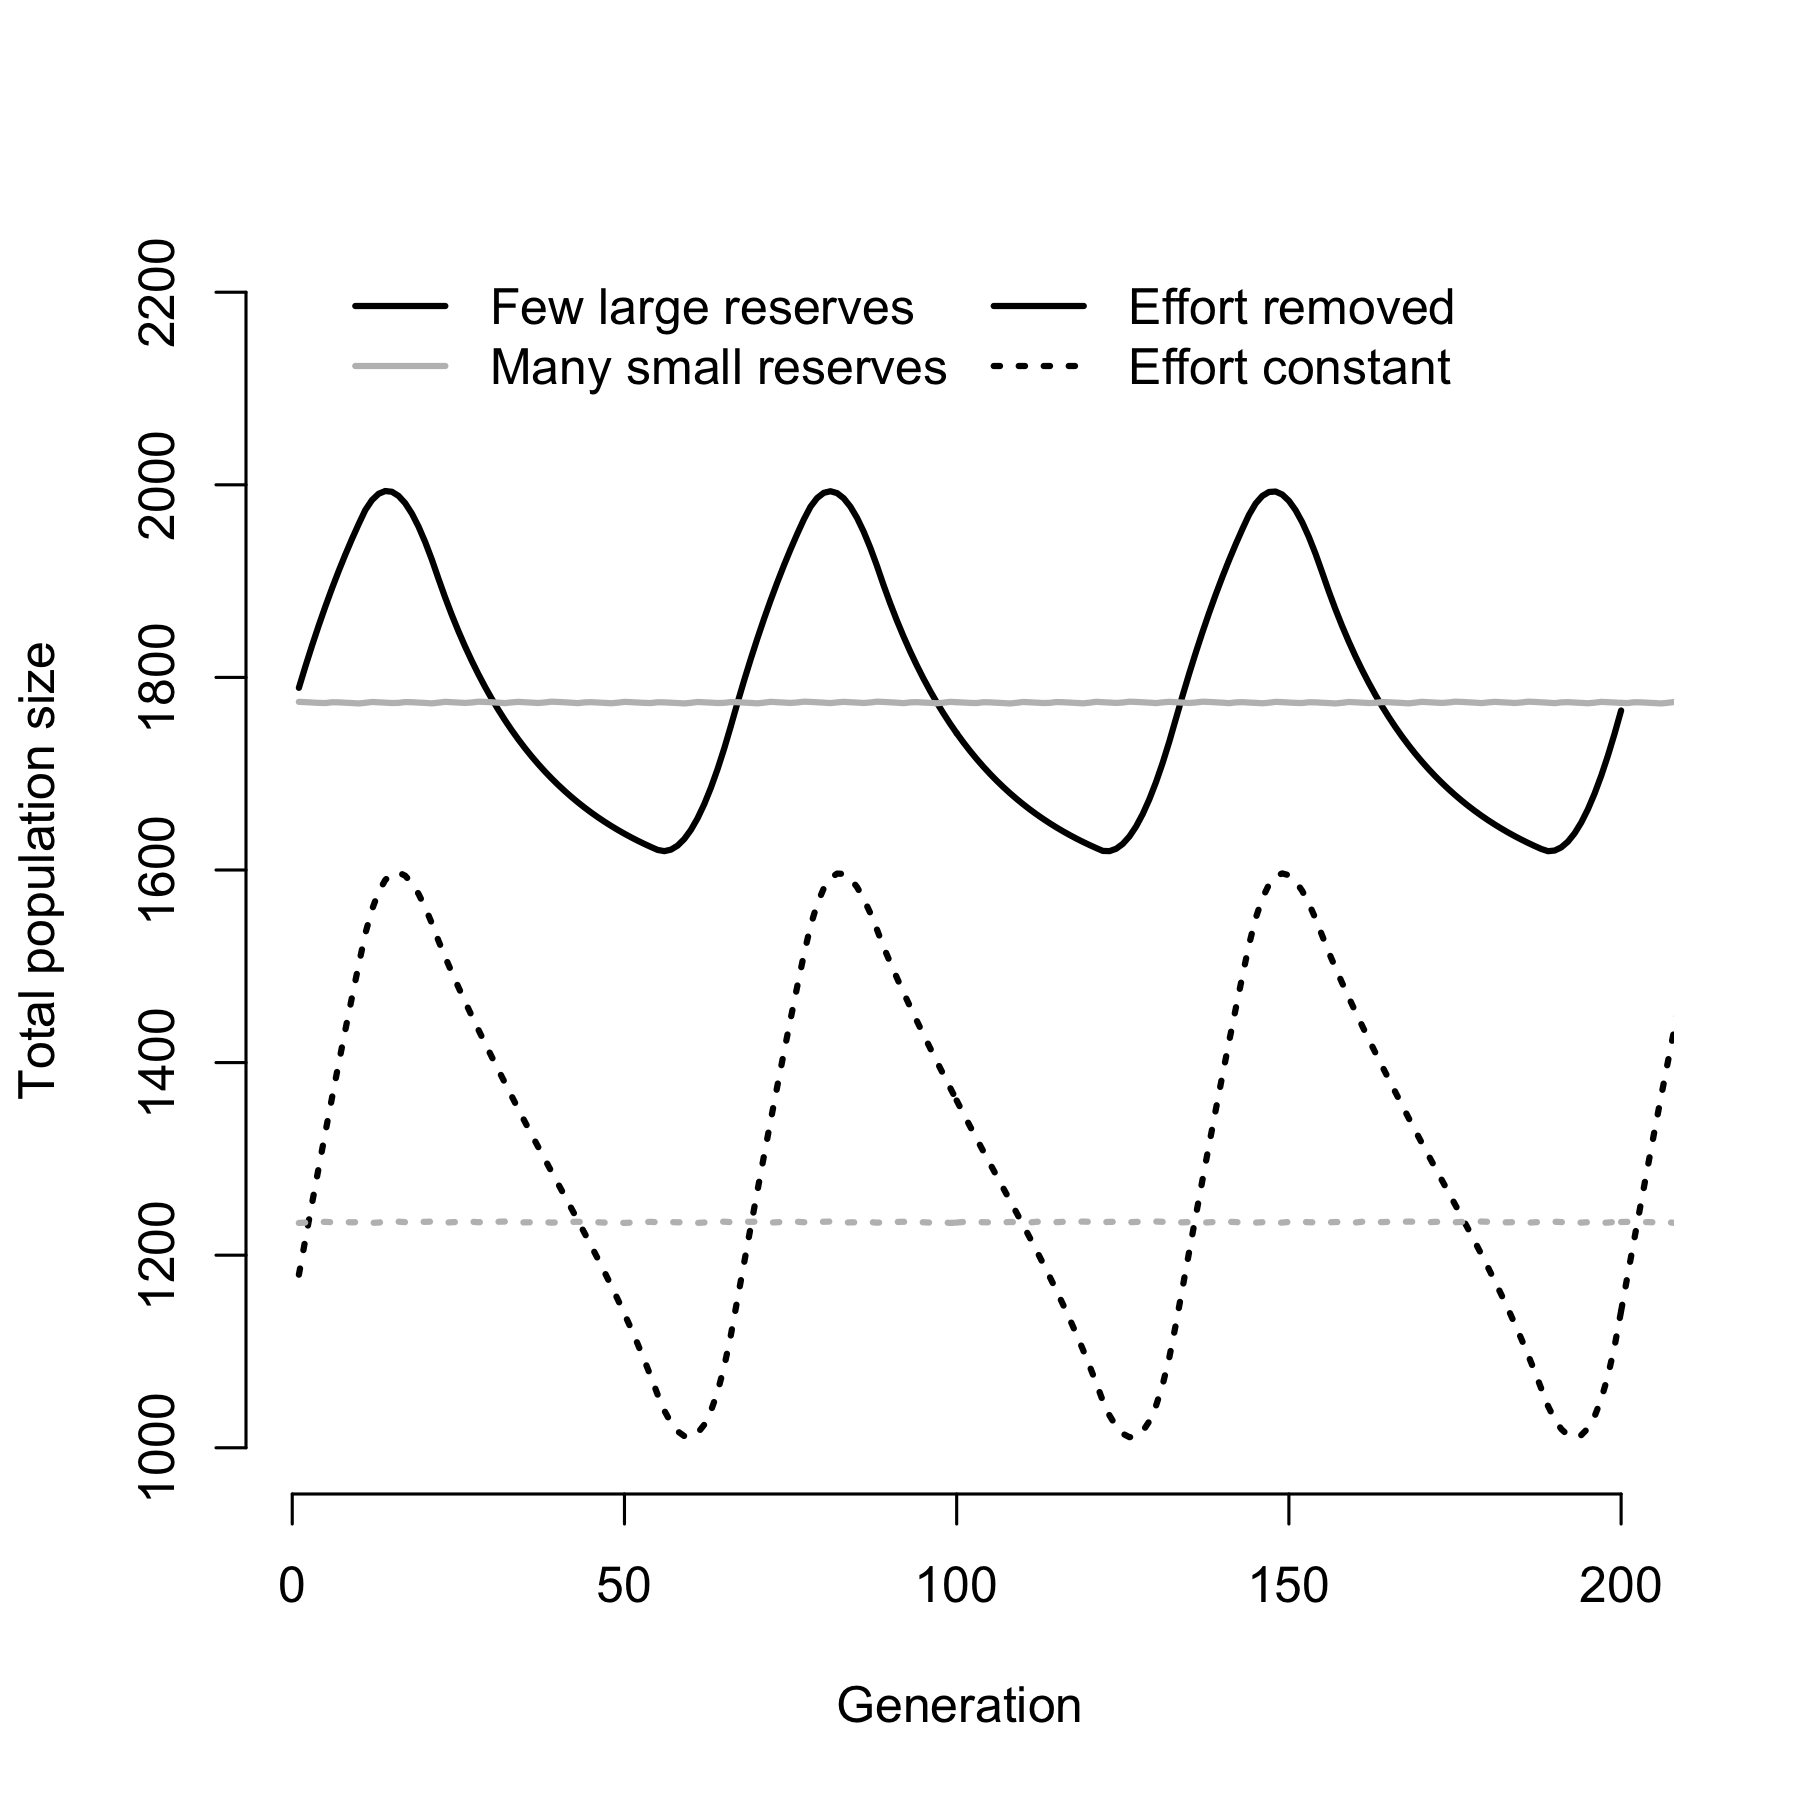
\includegraphics[width=.75\textwidth]{../../plots/compare_flucts.png}
\caption{\label{fluctuations} Total population biomass is on the y axis, and generation is on the x axis. These simulations were run with climate velocity $ = 0.1$, and a proportional harvest rate $= 0.02$. }
% see bounded\_flux.R for code that made this plot
\end{figure}

\begin{figure}[h]
\centering
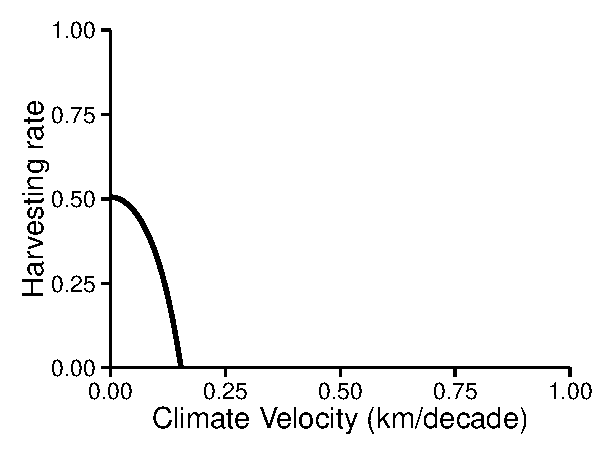
\includegraphics[width=.75\textwidth]{../../plots/rockfish_criticalh.pdf}
\caption{ \label{crith_rockfish}
Lines indicate the critical threshold for persistence as a function of harvest fraction on the y-axis and climate velocity on the x-axis. Model parameterized for black rockfish. }
 \end{figure}
 
 \begin{figure}[h]
 \centering
 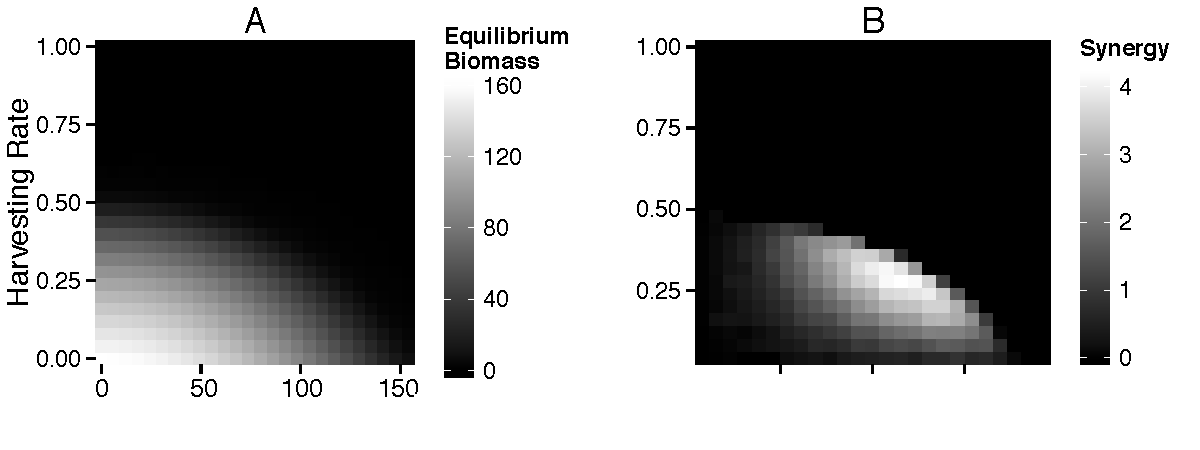
\includegraphics[width=.75\textwidth]{../../plots/rockfisheqbiomass.pdf}
 \caption{ \label{synergy_rockfish}
 (a) Results from a model parameterized for black rockfish. The equilibrium biomass of a black rockfish population as a function of the climate velocity on the x-axis and the harvest fraction on the y-axis. (b) Interaction between the two stressors as a function of climate velocity and harvest fraction. The heat map indicates the interaction measure $S$, i.e., the loss in biomass in the doubly stressed population in excess of the sum of the losses caused by each stressor individually ($E_{hc}-E_h-E_c$). $S$ of $0$ indicates additive interaction of the stressors. The excess loss, on the order of $4$, is small in comparison to the total biomass, which can be as large as $160$.
 }
 \end{figure}

\begin{figure}[h]
\centering
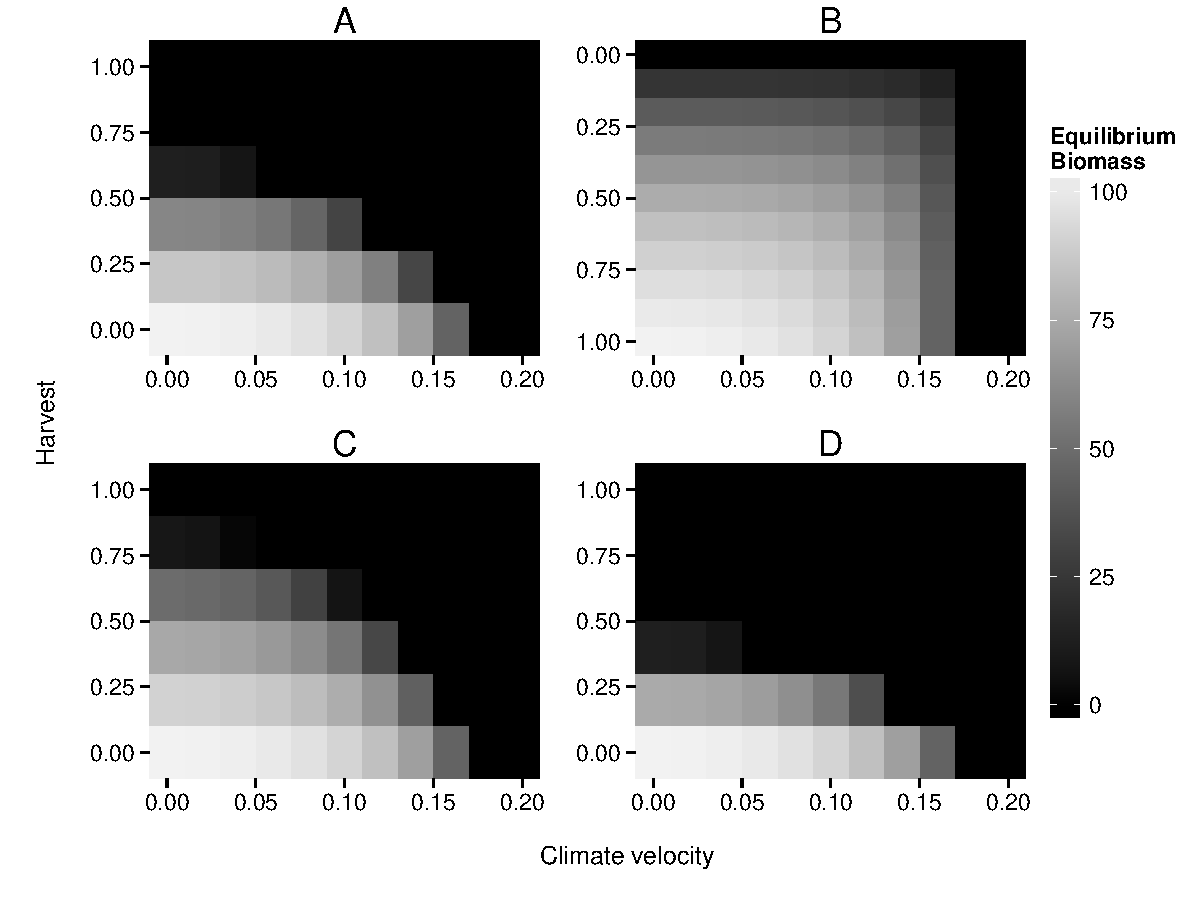
\includegraphics[width=.75\textwidth]{../../plots/rockfish_sims.pdf}
\caption{\label{simulation_rockfish} The equilibrium biomass of the population as a function of the climate velocity on the x-axis and the harvest fraction on the y-axis under alternative management strategies as parameterized for black rockfish. (a) The equilibrium biomass for simulations with constant harvest rates. (b) Equilibrium biomass for simulations with threshold management. For threshold management, we set a threshold density below which no fishing is allowed. The threshold ranges between 0 (no fishing allowed) and 1 (all fish taken), with intermediate density thresholds determined as fractions of the maximum population density observed at a given time step before harvesting. We show this on the y-axis. (c) Equilibrium biomass for simulations with protected areas where harvesting pressure outside reserves is unchanged  (i.e., harvest effort inside reserves is eliminated). (d) Equilibrium biomass for simulations with protected areas in which harvesting pressure is reallocated outside reserves.}
\end{figure}


\cleardoublepage

\bibstyle{cbe}
\bibliography{fish}

\end{document}